

\documentclass{article}
\usepackage[utf8]{inputenc}
\usepackage[utf8]{inputenc}
\usepackage[T1]{fontenc}
\usepackage[english]{babel}
\usepackage{fullpage}
\usepackage{color}
\usepackage[table]{xcolor}
\usepackage{listings}
 
\definecolor{darkWhite}{rgb}{0.94,0.94,0.94}
 
\lstset{
  aboveskip=3mm,
  belowskip=-2mm,
  backgroundcolor=\color{darkWhite},
  basicstyle=\footnotesize,
  breakatwhitespace=false,
  breaklines=true,
  captionpos=b,
  commentstyle=\color{red},
  deletekeywords={...},
  escapeinside={\%*}{*)},
  extendedchars=true,
  framexleftmargin=16pt,
  framextopmargin=3pt,
  framexbottommargin=6pt,
  frame=tb,
  keepspaces=true,
  keywordstyle=\color{blue},
  language=C,
  literate=
  {²}{{\textsuperscript{2}}}1
  {⁴}{{\textsuperscript{4}}}1
  {⁶}{{\textsuperscript{6}}}1
  {⁸}{{\textsuperscript{8}}}1
  {€}{{\euro{}}}1
  {é}{{\'e}}1
  {è}{{\`{e}}}1
  {ê}{{\^{e}}}1
  {ë}{{\¨{e}}}1
  {É}{{\'{E}}}1
  {Ê}{{\^{E}}}1
  {û}{{\^{u}}}1
  {ù}{{\`{u}}}1
  {â}{{\^{a}}}1
  {à}{{\`{a}}}1
  {á}{{\'{a}}}1
  {ã}{{\~{a}}}1
  {Á}{{\'{A}}}1
  {Â}{{\^{A}}}1
  {Ã}{{\~{A}}}1
  {ç}{{\c{c}}}1
  {Ç}{{\c{C}}}1
  {õ}{{\~{o}}}1
  {ó}{{\'{o}}}1
  {ô}{{\^{o}}}1
  {Õ}{{\~{O}}}1
  {Ó}{{\'{O}}}1
  {Ô}{{\^{O}}}1
  {î}{{\^{i}}}1
  {Î}{{\^{I}}}1
  {í}{{\'{i}}}1
  {Í}{{\~{Í}}}1,
  morekeywords={*,...},
  numbers=left,
  numbersep=10pt,
  numberstyle=\tiny\color{black},
  rulecolor=\color{black},
  showspaces=false,
  showstringspaces=false,
  showtabs=false,
  stepnumber=1,
  stringstyle=\color{gray},
  tabsize=4,
  title=\lstname,
}
\usepackage{graphicx}
\title{HAI804I – Codage et compression multimédia
}
\author{Fabien Caballero}

\begin{document}

\maketitle
    \tableofcontents

\newpage

\begin{figure}[h]
\centerline{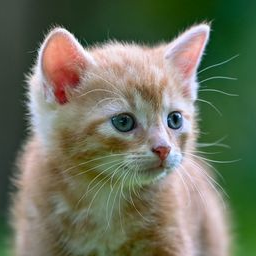
\includegraphics[scale=0.3]{./rendus/Chalex.png}}
\caption{Image d'origine utilisée tout le long du TP}
\end{figure}

\addcontentsline{toc}{section}{Introduction}
\section*{Introduction}
Le but de ce tp est d'observer l'impact de la réduction d'une image couleur sur la qualité.
Et de comparer cet impact en réduisant différentes composantes ou dans différents espaces.
\\\\
\section{Séparation des 3 composantes et réduction de 2 d'entres elles pour une image ppm}

\subsection{Séparation des composantes}
Pour récupérer chaques composantes il suffit de parcourir la taille de l'image est de prendre et de prendre la valeur i*3 si on veut le rouge, la i*3+1 pour le vert et la i*3+2 pour le bleu.

\begin{figure}[h]
\centerline{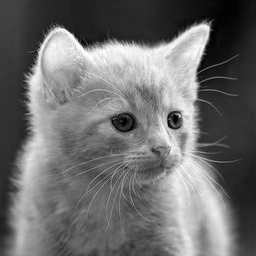
\includegraphics[scale=0.7]{./rendus/Red.png} 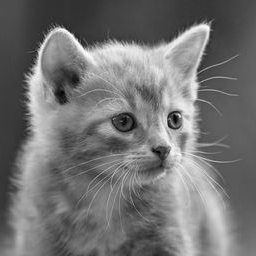
\includegraphics[scale=0.7]{./rendus/Green.png} 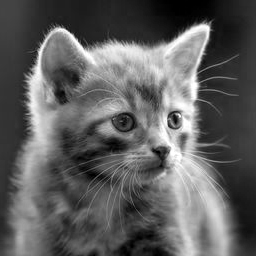
\includegraphics[scale=0.7]{./rendus/Blue.png} }
\caption{Composante Rouge, Verte et Bleue de l'image d'origine}
\end{figure}

\newpage
\subsection{réduction de 2 composantes}

Pour réduire une image il faut faire la moyenne de 4 pixels (formant un carré donc 2 sur la même ligne et 2 autres sur la ligne en dessous) et en faire 1 seul pixel dans l'image finale.
On parcours donc notre image de 0 à width/2 et de 0 à height/2.
Il faut penser que lorsque qu'on récupère les pixels de l'image d'origine et qu'on fait la moyenne il faut prendre 2 fois les coordonées i et j courantes puisque pour chaque pixel de l'image de sortie on prend 4 pixels de l'image d'entrée avec 2 sur chaque ligne, il nous faut donc faire une ligne sur 2 et avancer avec un pas de 2 pixels sur une ligne.
\\\\
Ensuite on les ré-assemble en utilisant nos 2 images réduites puis reconstruites à la place des composantes dont elles sont issues.
\subsubsection*{réduction de la composante verte et bleue}

\begin{figure}[h]
\centerline{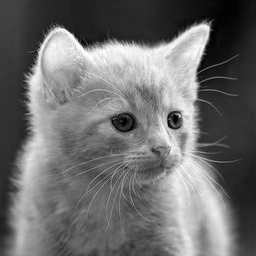
\includegraphics[scale=0.6]{./rendus/Red.png} 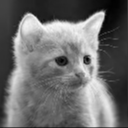
\includegraphics[scale=0.8]{./rendus/ReduceGreen.png} 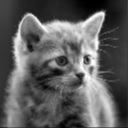
\includegraphics[scale=0.8]{./rendus/ReduceBlue1.png} }
\caption{Composante Rouge, Verte et Bleue de l'image d'origine, avec la composante verte et bleue réduite}
\end{figure}


\subsubsection*{réduction de la composante rouge et bleue}

\begin{figure}[h]
\centerline{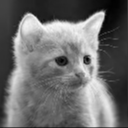
\includegraphics[scale=0.8]{./rendus/ReduceRed.png} 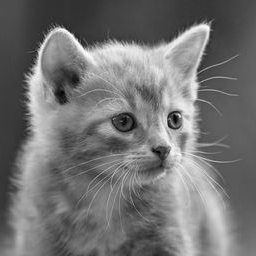
\includegraphics[scale=0.6]{./rendus/Green.png} 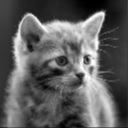
\includegraphics[scale=0.8]{./rendus/ReduceBlue.png} }
\caption{Composante Rouge, Verte et Bleue de l'image d'origine, avec la composante rouge et bleue réduite}
\end{figure}

\newpage
\section{Ré-échantillonage des 2 composantes réduites}
Pour le ré-échantillonage dans un premier temps on recopie sur 4 pixels de l'image de sortie la valeur d'un pixel de l'image réduite (toujours avec 2 pixels sur une ligne et 2 autres sur celle d'en dessous). Ensuite dans un second temps on fait la moyenne bicubique des voisins de chaque pixels et on affecte cette valeur à notre pixel courant.
On obtient ainsi une image de la taille originelle avec 4 fois moins d'informations ce qui rend celle-ci un peu floue.
\subsection{Avec les composantes verte et bleue réduites}

\begin{figure}[h]
\centerline{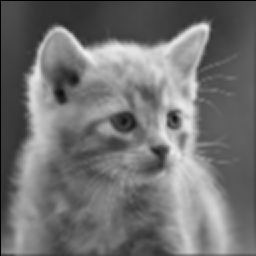
\includegraphics[scale=0.7]{./rendus/ResizeGreen.png} 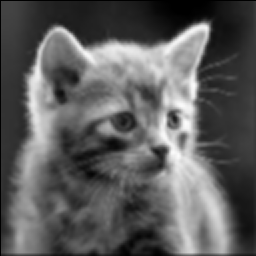
\includegraphics[scale=0.7]{./rendus/ResizeBlue.png} }
\caption{Composante Verte et Bleue ré-échantillonée }
\end{figure}

\subsubsection*{ré-assemblage des 3 composantes, avec les images précdentes}
\begin{figure}[h]
\centerline{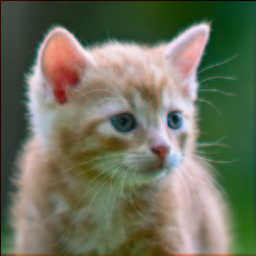
\includegraphics[scale=0.9]{./rendus/ChalexRGReduit.png} 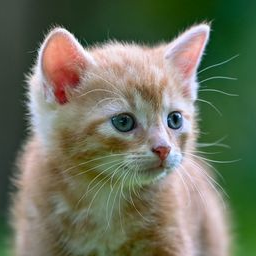
\includegraphics[scale=0.9]{./rendus/Chalex.png} }
\caption{Image reconstruite (gauche) et image d'origine (droite) }
\end{figure}

PSNR de 29.7921 dB


\newpage
\subsection{Avec les composantes rouge et bleue réduites}
\begin{figure}[h]
\centerline{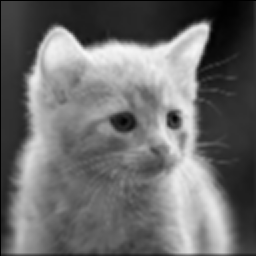
\includegraphics[scale=0.7]{./rendus/ResizeRed.png} 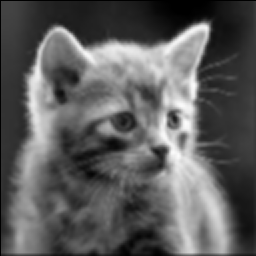
\includegraphics[scale=0.7]{./rendus/ResizeBlue.png} }
\caption{Composante Rouge et Bleue ré-échantillonée }
\end{figure}

\subsubsection*{ré-assemblage des 3 composantes, avec les images précdentes}
\begin{figure}[h]
\centerline{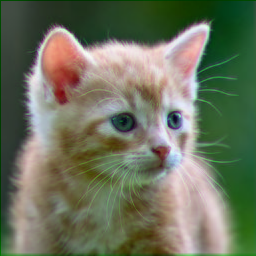
\includegraphics[scale=0.9]{./rendus/ChalexRBReduit.png} 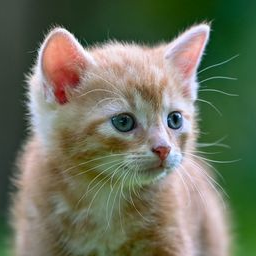
\includegraphics[scale=0.9]{./rendus/Chalex.png} }
\caption{Image reconstruite (gauche) et image d'origine (droite) }
\end{figure}

PSNR 29.6275 dB

\section{Application à une image YCrCb en réduisant Cr et Cb}



\subsection{création des composantes Y,Cr et Cb}

Pour l'appliquer a un espace YCrCb on transforme notre image RGB en YCrCb en utilisant les coefficient de proportion de R de G et de B pour le Y, le Cr et le Cb.

\begin{figure}[h]
\centerline{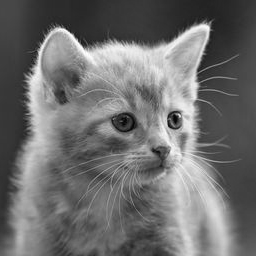
\includegraphics[scale=0.7]{./rendus/Y.png} 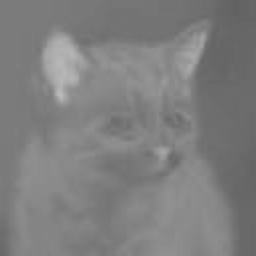
\includegraphics[scale=0.7]{./rendus/Cr.png} 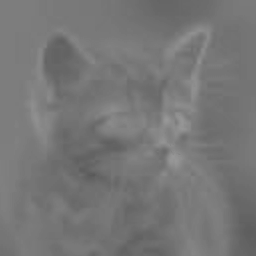
\includegraphics[scale=0.7]{./rendus/Cb.png}}
\caption{Composante Y, Cr et Cb }
\end{figure}

Même principe que pour l'esapce RGB

\subsection{Réduction des composantes Cr et Cb réduites}
\begin{figure}[h]
\centerline{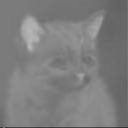
\includegraphics[scale=1.5]{./rendus/ReduceCr.png} 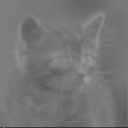
\includegraphics[scale=1.5]{./rendus/ReduceCb.png} }
\caption{Composante Cr et Cb réduites }
\end{figure}

Même principe que pour l'esapce RGB

\newpage
\subsubsection*{ré-échantillonage de Cr et Cb}
\begin{figure}[h]
\centerline{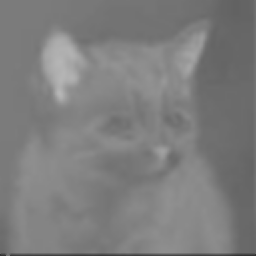
\includegraphics[scale=0.9]{./rendus/ResizeCr.png} 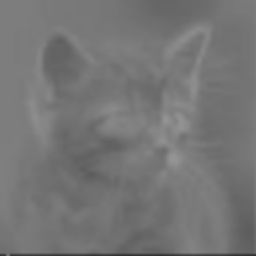
\includegraphics[scale=0.9]{./rendus/ResizeCb.png} }
\caption{Composante Cr et Cb ré-échantillonées}
\end{figure}

Puis on reconvertit en RGB toujours avec les coefficient adaptés à la reconversion.

\newpage
\subsubsection*{Conversion de l'image dans l'espace YCrCb en RGB}
\begin{figure}[h]
\centerline{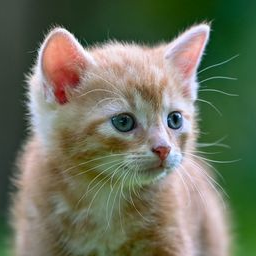
\includegraphics[scale=0.9]{./rendus/Chalex.png} 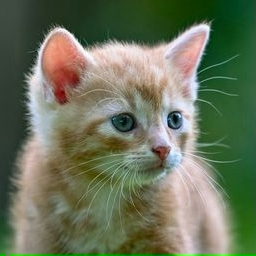
\includegraphics[scale=0.9]{./rendus/ChalexYCrCbReduit.png} }
\caption{Image reconstruite (gauche) et image d'origine (droite) }
\end{figure}


PSNR de 31.4582 dB


\addcontentsline{toc}{section}{Conclusion}
\section*{Conclusion}

On en conclu que la réduction et reconstruction est plus qualitative lorsque qu'on réduit le Cr et le Cb de notre image dans l'espace YCrCb et qu'on la reconvertit ensuite en RGB.
Cela est dû au fait que la chrominance n'as pas le même poids que le rouge ou le bleu.
En effet dans l'espace RGB chaque composante est codée sur 1 octet donc chaque composante a le même poids dans la couleur d'un pixel, alors que dans l'esapce YCrCb la luminance est codée sur 1 octet et Cr et Cb sont codés sur un octet donc chacune sur 4 bits.
Étant donné que le poids de la chrominance est plus faible que que celui d'une composante de RGB, la dégradation sur la qualité, lors de la réduction et de la reconstruction sera aussi plus faible.
\\\\

On peut utiliser une autre approche comme la détection de patterns de succesions de couleurs dans une image, avec par exemple un certain écart autorisé. On pourrait ainsi construire l'image d'origine (avec perte potentiellement), à partir d'une image réduite composée des index des patterns à insérer, et d'une table de patterns.

D'autres méthodes peuvent être utilisées pour compresser une image et obtenir un taux de compression de 2 comme l'algorithme de JPEG2000 ou le LZMA selon la taille de codage des couleurs, ou encore utilisée une squeletisation, avec détection de similaritées pour des images de manuscrits.

source: https://www.lirmm.fr/coresa2007/PDF/43.pdf
\\\\
Ce Tp m'a permis d'observer une réduction, une reconstruction puis de la mettre en pratique. Celui-ci était intéréssant de voir les imapct que la réduction peut avoir selon l'espace dans lequel on se trouve.



\end{document}